% minimalist greeting card document using gcard package
% Sets text in 12 pt CMR (not exactly traditional for cards!)
% G. C. McBane  21 May 2007
\documentclass[12 pt]{article}
\usepackage{gcard}
\usepackage{mathrsfs}
\usepackage{amsmath}
\usepackage{caption}
\usepackage{mathtools}
\begin{document}

\begin{frontcover}
%
\textit{Question 1: Indefinite Limits} \\ 
%
\\~\\
Let $s$ be a student of age 23 years living a distance $d$ from his family, a set $\mathcal{F}$ with $N$ members, $f_i$. Let $\mathcal{L}_s(x)$ be a function of the magnitude of love, $l$, the student $s$ has for his family that takes a distance argument, $x$.  Compute the limit of the student's love as a function using the distance measure $\delta(x)$, that is 
%
\begin{equation*}
\lim_{x\to{d}}\int_{\mathcal{F}}{\mathcal{L}_s(x)\delta(x)} 
\end{equation*}
%
\end{frontcover}
%
\begin{backcover}
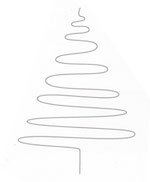
\includegraphics[width=\panelwidth]{tree.jpg}
\centering
\Large{merry christmas} $\heartsuit$
\end{backcover}
%
\begin{insideright}
\textit{Solution 1: Indefinite Limits} \\ 
%
\\~\\
First, we write down the integral of the function with correct limits and notice that we can split the integral into components where 
%
\begin{equation*}
\int_{\mathcal{F}}\mathcal{L}_s(x)\delta(x) = 
\sum_{i=1}^{N}\int_{f_i}{\mathcal{L}_s(x)\delta(x)}
\end{equation*}
%
such that each integral can be evaulated for each of the N family members. By thinking of the nature of the function $\mathcal{L}$ we realize there exists a singularity with respect to $x$ which results in a rapid divergence at distance $d$. That is, for each family member, love goes to infinity at any distance. 
%
\begin{equation*}
\lim_{x\to{d}}\int_{\mathcal{F}}{\mathcal{L}_s(x)\delta(x)} \to \infty 
\end{equation*}
%
\centering$\heartsuit$
%
\end{insideright}

\end{document}